\documentclass[border=2pt]{standalone}
\usepackage[T1]{fontenc}
\usepackage{helvet}
\renewcommand{\familydefault}{\sfdefault}
\usepackage{amsmath,amssymb}
\usepackage{tikz}
\usetikzlibrary{positioning,arrows.meta,calc}
\definecolor{ink}{HTML}{0B0B0B}\definecolor{muted}{HTML}{52514E}
\definecolor{blue}{HTML}{2A78D6}\definecolor{lblue}{HTML}{E6EFFA}
\definecolor{orange}{HTML}{EB6834}\definecolor{lorange}{HTML}{FCE9E1}
\begin{document}
\hyphenpenalty=10000\exhyphenpenalty=10000
% Final width about 130 mm, the text width of the journal, so \footnotesize prints at 8 pt.
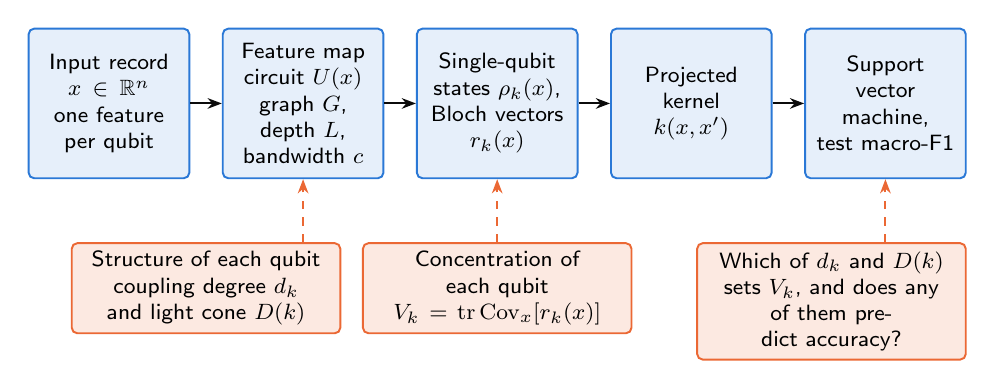
\begin{tikzpicture}[font=\footnotesize, >={Stealth[length=1.8mm]},
  box/.style={draw=blue, fill=lblue, rounded corners=2pt, minimum height=19mm, text width=19mm, align=center, inner sep=2pt, line width=0.7pt},
  note/.style={draw=orange, fill=lorange, rounded corners=2pt, text width=32mm, align=center, inner sep=3pt, line width=0.7pt}]
\node[box] (x) {Input record\\ $x\in\mathbb{R}^{n}$\\ one feature\\ per qubit};
\node[box, right=4mm of x] (u) {Feature map\\ circuit $U(x)$\\ graph $G$,\\ depth $L$,\\ bandwidth $c$};
\node[box, right=4mm of u] (r) {Single-qubit\\ states $\rho_k(x)$,\\ Bloch vectors\\ $r_k(x)$};
\node[box, right=4mm of r] (k) {Projected\\ kernel\\ $k(x,x')$};
\node[box, right=4mm of k] (f) {Support\\ vector\\ machine,\\ test macro-F1};
\foreach \a/\b in {x/u,u/r,r/k,k/f} \draw[->, draw=ink, line width=0.7pt] (\a) -- (\b);
\node[note, below=8mm of $(x.south)!0.5!(u.south)$, anchor=north] (n1) {Structure of each qubit\\ coupling degree $d_k$\\ and light cone $D(k)$};
\node[note, below=8mm of r.south, anchor=north] (n2) {Concentration of\\ each qubit\\ $V_k=\operatorname{tr}\operatorname{Cov}_x[r_k(x)]$};
\node[note, below=8mm of f.south east, anchor=north east] (n3) {Which of $d_k$ and $D(k)$\\ sets $V_k$, and does any\\ of them predict accuracy?};
\draw[->, dashed, orange, line width=0.7pt] (n1.north -| u.south) -- (u.south);
\draw[->, dashed, orange, line width=0.7pt] (n2.north -| r.south) -- (r.south);
\draw[->, dashed, orange, line width=0.7pt] (n3.north -| f.south) -- (f.south);
\end{tikzpicture}
\end{document}
